% 07_masses.tex -- Part 7, electron and hole masses. Sources: research_monograph/chapters/M09_masses_parameters.tex
% (sec:mono-mass-bulk, sec:mono-mass-electrons, sec:mono-mass-holes, tab:mono-mass-laws, tab:mono-mass-tcad),
% M05_confinement_theory.tex (sec:mono-conf-kane, sec:mono-conf-subband, sec:mono-conf-test, tab:mono-conf-test),
% M03_literature_materials.tex (sec:mono-lit-mass), evidence/FACT_REGISTRY.tsv (FACT-004, 005, 006, 026a-d, 027, 047,
% 060, 061, 062), evidence/CLAIM_SOURCE_MAP.tsv (C039, C040, M004), evidence/derived/confinement_analysis.json,
% appendices/MG_corrections.tex (X6, V5, V10), qe_workflow/cern_htcondor/results/RESULTS_LOG.md (2026-10-14 entry),
% qe_workflow/analysis_2026-10-13_full/bands_masses/BANDS_MASSES.md (section 2.3 checks), chapters/13_dft_rev.tex
% (experimental lattice 10.117 A).
% Figures: tools/fig_07_masses.py (data: qe_workflow/analysis_2026-10-13_full/bands_masses/out/b01_masses.json,
% b03_gaps_laws.json, b05_holes.json; evidence/derived/confinement_analysis.json).
% Note: frame bodies start with a command, never with a brace group (beamer would read a subtitle).
% denser slides: footnotesize bullets, local to the frame in which it is called
\providecommand{\sevdense}{\setbeamerfont{itemize/enumerate body}{size=\footnotesize}%
  \setbeamerfont{itemize/enumerate subbody}{size=\footnotesize}}
% evidence label inside a \src line: same vocabulary as \lab, but at the (tiny) size of the source line
\providecommand{\sevsrclab}[1]{[\textsc{\MakeLowercase{#1}}]}
\providecommand{\sevNv}{N_{\mathrm{v}}}
% pull the frame body up towards the title rule (as in Parts 5 and 8); keeps clear space above the take-away
\providecommand{\sevTop}{\vspace{-3mm}}

\partslide{Part 7}{Electron and hole masses}

% ---------------------------------------------------------------------------------------------------------------------
\begin{frame}{Bulk electrons: a Kane band, 26\,\% lighter than measured}
  \sevdense\sevTop
  \begin{columns}[T,onlytextwidth]
    \begin{column}{0.47\textwidth}
      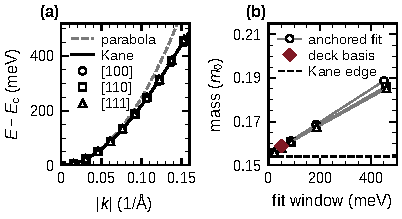
\includegraphics[width=\linewidth]{07_bulk_cb}
      \src{(a) Bulk conduction band near $\Gamma$; solid: Kane band; dashed: parabola, same $m_b$. (b) Mass by fit
        basis: parabolas anchored at $\Gamma$ over 25--450\,meV windows, four-point deck basis, Kane band edge. This work,
        PAW-PBE \sevsrclab{computed}.}
    \end{column}
    \begin{column}{0.49\textwidth}
      \begin{itemize}
        \item $E(1+\alpha E) = \hbar^2k^2/2m_b$ fits [100], [110], [111] to 0.45\,eV: $m_b$ = 0.1541\,$m_0$ (isotropic
          within 0.2\,\%), $\alpha$ = 0.58\,eV$^{-1}$ (0.55--0.63). Other bases: four-point (deck) 0.1588\,$m_0$,
          anchored parabolas 0.156--0.189\,$m_0$ \lab{computed}.
        \item Measured: 0.208\,$\pm$\,0.006\,$m_0$\sref[p.~225102-1]{Stokey2021}; 0.18\,$m_0$ at zero density, about 0.4\,$m_0$ at
          $10^{21}$\cmcu\sref{Feneberg2016} \lab{measured}; PBE Kane optical mass $m_b(1+2\alpha\EF)$ there
          0.39\,$m_0$ ($\EF$ beyond the fit window) \lab{derived}.
        \item Caveats: a polaron (Fr\"ohlich coupling near one: +15\,\%) could explain half of the 26\,\%
          \lab{hypothesis}; the two-band gap is not the fundamental one (dipole-forbidden edge\sref{Walsh2008}).
      \end{itemize}
    \end{column}
  \end{columns}
  \takeaway{Decks: measured 0.208\,$m_0$ plus the PBE increase on the deck basis, 0.1114\,$t^{-1.2611}$\,$m_0$.}
\end{frame}

% ---------------------------------------------------------------------------------------------------------------------
\begin{frame}{Confinement raises the mass; extrapolated, little beyond 2\,nm}
  \sevdense\sevTop
  \begin{columns}[T,onlytextwidth]
    \begin{column}{0.43\textwidth}
      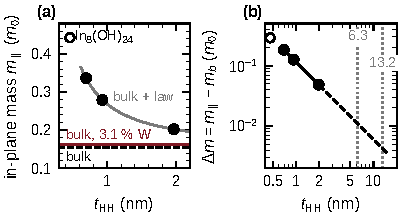
\includegraphics[width=\linewidth]{07_film_masses}
      \src{(a) In-plane band-edge mass of the relaxed films. (b) Increase over bulk with the fitted law; dashed:
        extrapolated. Open: In$_8$(OH)$_{24}$, outside every law. This work, PAW-PBE \sevsrclab{computed},
        law \sevsrclab{fitted}.}
    \end{column}
    \begin{column}{0.53\textwidth}
      \begin{itemize}
        \item In-plane band-edge masses (2-D DOS, Kane basis): 0.443, 0.337, 0.279, 0.203\,$m_0$ from 0.461 to
          1.962\,nm; in-plane $\alpha$ 0.24--0.47\,eV$^{-1}$ \lab{computed}.
        \item Fit, 0.695--1.962\,nm, one residual degree of freedom, band-edge basis: $\Delta m$ =
          0.1145\,$t^{-1.2755}$\,$m_0$ ($t = \tHH$ in nm); 0.047\,$m_0$ at 2.0\,nm \lab{fitted}.
        \item The device decks use the deck-basis law 0.1114\,$t^{-1.2611}$\,$m_0$ (previous slide); both laws
          give 0.011 and 0.004\,$m_0$ at 6.3 and 13.2\,nm, extrapolated \lab{fitted}.
        \item Deck basis at 2\,nm: 0.206\,$m_0$. Checks: GPU against CPU 0.0006\,$m_0$, 15--35\,\AA{} vacuum
          0.0002\,$m_0$; relaxation: +18\,\% at 1\,nm \lab{computed}.
        \item 3.1\,\% W in bulk: same shape, 5\,\% heavier, 0.161--0.163\,$m_0$ \lab{computed}; no W-film band run.
      \end{itemize}
    \end{column}
  \end{columns}
  \takeaway{Beyond 2\,nm confinement adds little to the electron mass: 0.011\,$m_0$ at 6.3\,nm \lab{fitted}.}
\end{frame}

% ---------------------------------------------------------------------------------------------------------------------
\begin{frame}{No-fit Kane test: 1\,\% off at 2\,nm, 10\,\% off at 1\,nm}
  \sevdense\sevTop
  \begingroup\small\setlength{\abovedisplayskip}{2pt}\setlength{\belowdisplayskip}{2pt}%
  Kane band\sref{Kane1957} confined with $k_z = n\pi/t$, expanded at $k_\parallel = 0$:
  \begin{equation*}
    E(1+\alpha E) = \varepsilon_n + \frac{\hbar^2k_\parallel^2}{2m_b},\quad
    \varepsilon_n = \frac{\hbar^2\pi^2n^2}{2m_bt^2}
    \quad\Longrightarrow\quad
    m_\parallel = m_b\,(1+2\alpha E_1),\quad \alpha_\parallel = \frac{\alpha}{1+2\alpha E_1}
  \end{equation*}
  where $E_1$ = computed $\dEc$; bulk fit (to 0.45\,eV) $m_b$ = 0.1541\,$m_0$, $\alpha$ = 0.58\,eV$^{-1}$: nothing
  is adjusted.\par\endgroup
  \vspace{1mm}
  \begin{columns}[T,onlytextwidth]
    \begin{column}{0.47\textwidth}
      \begingroup\scriptsize
      \setlength{\tabcolsep}{3.2pt}
      \renewcommand{\arraystretch}{1.1}
      \begin{tabular*}{\linewidth}{@{\extracolsep{\fill}}l c c c r@{}}
        \toprule
        $\tHH$ (nm) & $\dEc$ (eV) & $m_\parallel$ comp. & $m_\parallel$ Kane & Kane/comp.\,\textminus\,1 \\
        \midrule
        1.962 & 0.281 & 0.203 & 0.204 & +0.7\,\% \\
        0.930 & 0.848 & 0.279 & 0.306 & +9.6\,\% \\
        0.695$^a$ & 1.059 & 0.337 & 0.343 & +1.9\,\% \\
        0.461$^b$ & 1.585 & 0.443 & 0.437 & \textminus1.3\,\% \\
        \bottomrule
      \end{tabular*}\par\endgroup
      \src{Masses in $m_0$; comp.: computed in-plane 2-D DOS band-edge mass. $^a$Polar film, $\dEc$ \textpm\,0.17\,eV.
        $^b$In$_8$(OH)$_{24}$. FACT-027 \sevsrclab{derived}.}
    \end{column}
    \begin{column}{0.49\textwidth}
      \begin{itemize}
        \item Tests: 1.962 and 0.930\,nm. The 0.930\,nm test uses the band at 0.85\,eV, beyond the fit window; the
          two-step $\dEc$ (0.819\,eV) still gives 0.300\,$m_0$ \lab{derived}.
        \item The 0.695 and 0.461\,nm films agree within 2\,\% but do not test it: 1.585\,eV is far beyond the fit
          window, and \textpm0.17\,eV moves the 0.695\,nm prediction by \textpm9\,\%.
      \end{itemize}
    \end{column}
  \end{columns}
  \takeaway{At 2\,nm the mass increase is consistent, within 1\,\%, with the bulk non-parabolicity at the subband
    energy \lab{derived}.}
\end{frame}

% ---------------------------------------------------------------------------------------------------------------------
\begin{frame}{The mass law and the $\dEc$ law are one input, not two}
  \sevdense\sevTop
  \begin{columns}[T,onlytextwidth]
    \begin{column}{0.47\textwidth}
      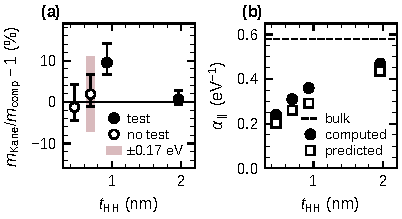
\includegraphics[width=\linewidth]{07_kanetest}
      \src{(a) Kane prediction against the computed in-plane mass; bars: $\alpha$ = 0.55--0.63; shaded: \textpm0.17\,eV
        in the polar 0.695\,nm film; open: no test. (b) In-plane non-parabolicity, computed and $\alpha/(1+2\alpha
        E_1)$. This work \sevsrclab{derived}. Claim M004; review correction V5.}
    \end{column}
    \begin{column}{0.49\textwidth}
      \begin{itemize}
        \item The bulk $\alpha$ range (bars) moves the 0.930\,nm prediction only to 0.298--0.319\,$m_0$, against
          0.279\,$m_0$ computed \lab{derived}.
        \item $\alpha/(1+2\alpha E_1)$ lies 7--19\,\% below the computed $\alpha_\parallel$, with the right trend
          \lab{derived}.
        \item The total in-plane mass follows from $\dEc$ within 10\,\%, $\Delta m$ itself within about 20\,\%; the
          fitted exponents, 1.28 ($\Delta m$) and 1.48 ($\dEc$), diverge when extrapolated \lab{derived}.
        \item A device model that uses both laws therefore carries one independent first-principles input, not two
          (Part~10).
      \end{itemize}
    \end{column}
  \end{columns}
  \takeaway{The two laws are one input; at 6.3 and 13.2\,nm both are extrapolated \lab{derived}.}
\end{frame}

% ---------------------------------------------------------------------------------------------------------------------
\begin{frame}{No single hole mass; \textit{N}\textsubscript{v} is about 200 times the deck value}
  \sevdense\sevTop
  \begin{columns}[T,onlytextwidth]
    \begin{column}{0.47\textwidth}
      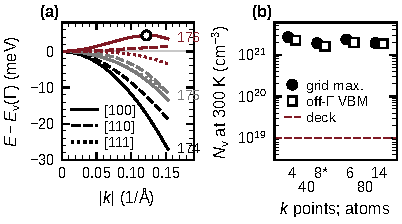
\includegraphics[width=\linewidth]{07_holes}
      \src{(a) Valence bands near $\Gamma$; circle: global maximum. (b) $\sevNv$ from the Boltzmann-integrated valence
        DOS, two energy references; $k$-mesh convergence not established. Grids: 40-atom primitive cell, 4 and 8 $k$
        points ($^*$at the experimental lattice, 10.117\,\AA); 80-atom cell, 6 and 14 $k$ points. Dashed: deck value.
        This work, PAW-PBE \sevsrclab{computed}.}
    \end{column}
    \begin{column}{0.49\textwidth}
      \begin{itemize}
        \item Three-fold degenerate top with a 4.4\,meV camel back (${\ll}\,\kT$). Curvature masses
          3.2--7.9\,$m_0$ (band 174), 6.9--19.8\,$m_0$ (175); band 176 rises along [100] and [110] \lab{computed}.
        \item Valence DOS: $\sevNv$ = 1.6--2.7\,$\times$\,$10^{21}$\cmcu{} (300\,K), $m_{h,\mathrm{DOS}}$ =
          16--22\,$m_0$; $k$-mesh convergence not established \lab{computed}.
        \item Decks: $\sevNv = 10^{19}$\cmcu{} (0.54\,$m_0$), electrons only \lab{assumed}.
        \item Computed $\sevNv$: $n_i$ (2\,nm) rises from 5.0\,$\times$\,$10^{-10}$ to 6.7\,$\times$\,$10^{-9}$\cmcu;
          equilibrium SRH generation ${\le}$\,3.4\,$\times$\,$10^{-3}$\,cm$^{-3}$\,s$^{-1}$, negligible \lab{derived}.
        \item Holes are predicted to self-trap\sref{Varley2012}; $\sevNv$ is a free-hole band integral.
      \end{itemize}
    \end{column}
  \end{columns}
  \takeaway{Only $\sevNv$ is usable for holes; in the electron-only decks its effect is negligible \lab{derived}.}
\end{frame}
